\documentclass[12pt,a4paper]{ctexart}
\usepackage[margin=2.2cm]{geometry}
\usepackage{graphicx}
\usepackage{booktabs}
\usepackage{amsmath}
\usepackage{float}
\usepackage{hyperref}
\usepackage{xcolor}
\usepackage{listings}

\lstdefinelanguage{MIPSAsm}{
	morekeywords={ADD,ADDI,ADDIU,SUB,LW,SW,BEQ,TEQ},
	sensitive=true,
	morecomment=[l]{;},
	morestring=[b]"
}

\lstset{
	language=MIPSAsm,
	basicstyle=\ttfamily\small,
	keywordstyle=\color{blue!70!black},
	commentstyle=\color{green!40!black},
	stringstyle=\color{orange!60!black},
	showstringspaces=false,
	breaklines=true,
	frame=single,
	tabsize=4
}

\newcommand{\reporttitle}{上机试验1：流水线性能分析I}
\newcommand{\subtask}{MIPSsim与WinDLX流水线冲突分析}
\newcommand{\authname}{姓名}
\newcommand{\authid}{学号}

\title{\reporttitle}
\author{\authname：\underline{李祥熙} \quad \authid：\underline{2234412799}}
\date{\today}

\begin{document}
\maketitle

\section{实验目的}
本实验围绕5级MIPS流水线展开，目标如下：
\begin{itemize}
	\item 加深对MIPS五级流水线（IF/ID/EX/MEM/WB）工作机制的理解。
	\item 理解数据相关与控制相关对流水线停顿（stall）的影响。
	\item 通过设计不同指令组合，分别构造无冲突、RAW冲突、分支跳转三种场景并进行性能分析。
	\item 对比定向路径（Forwarding）开启与关闭时的统计差异，理解硬件优化效果。
\end{itemize}

\section{实验过程}
\subsection{实验环境}
\begin{itemize}
	\item 操作系统：Windows
	\item 汇编架构：MIPS（5级流水）
	\item 模拟器A：MIPSsim
	\item 模拟器B：WinDLX（用于定向路径开/关对比）
\end{itemize}

\subsection{实验步骤}
\begin{enumerate}
    \item 按照文档\texttt{wdlx tutorial.pdf}的说明，使用win31虚拟机，在启用和关闭Forwarding的两种情况下运行，并提供性能分析结果。
	\item 编写并调试三份汇编程序：\texttt{no\_hazard.s}、\texttt{raw\_hazard.s}、\texttt{branch\_jump.s}。
	\item 在MIPSsim中分别加载运行，记录时钟周期图与统计信息。
	\item 在WinDLX中进行Forwarding enabled/disabled两组运行并截取统计图。
	\item 根据截图中的周期数、停顿类型与分支统计，完成图文分析。
\end{enumerate}

\section{实验内容}

\subsection{Win31虚拟机：WinDXL开启和关闭Forwarding的性能对比}
Forwarding 功能通过在硬件中增加特殊的通路，允许指令在计算完成（通常是在 执行阶段 EX 或 访存阶段 MEM）后，直接将结果“转发”给流水线中后续需要的指令，而不必等待该结果写回到寄存器堆。

如果关闭Forwarding功能，为了保证逻辑正确，CPU 必须通过插入 暂停周期 (Stalls) 来等待数据写回，产生大量的流水线空泡。而开启Forwarding功能则消除或减少了因“写后读（RAW）”相关引起的停顿，使指令流更顺畅。

按照文档\texttt{wdlx tutorial.pdf}的说明，在启用和关闭Forwarding功能的情况下运行示例程序\texttt{fact.s}计算20的阶乘，在程序运行结束后，查看运行的统计数据，比较两种情况下运行的周期数和停顿数区别。

\subsection{场景一：无冲突流水线（no\_hazard.s）}
程序核心思路是先连续装载地址和数据，再进行两次加法与存储。关键点在于把可能的数据依赖拉开距离，尽量避免紧邻的load-use相关。

源码简要说明：
\begin{itemize}
	\item 前5条\texttt{ADDIU}把数据标签地址装入\texttt{\$r8\textasciitilde\$r12}。
	\item 三条\texttt{LW}将\texttt{A,B,C}读入寄存器。
	\item 两条\texttt{ADD}计算\texttt{A+B}和\texttt{B+C}，再用\texttt{SW}写回结果。
	\item 末尾\texttt{TEQ \$r0,\$r0}作为程序停止标记。
\end{itemize}

\subsection{场景二：RAW冲突（raw\_hazard.s）}
该程序故意构造了典型load-use依赖：先\texttt{LW \$r1,0(\$r9)}，紧接着\texttt{ADD \$r2,\$r1,\$r3}读取\texttt{\$r1}，因此会触发RAW相关停顿。

源码简要说明：
\begin{itemize}
	\item \texttt{INC}与\texttt{VAL}分别加载到\texttt{\$r3}和\texttt{\$r1}。
	\item \texttt{ADD}直接消费刚load的\texttt{\$r1}，用于演示RAW。
	\item \texttt{SW}把结果写入\texttt{OUT}，便于验证正确性。
\end{itemize}

\subsection{场景三：分支跳转（branch\_jump.s）}
该程序包含\texttt{BEQ \$r1,\$r0,DO\_ADD}。由于\texttt{FLAG=0}，分支被取走，形成一次明确的控制相关场景。

源码简要说明：
\begin{itemize}
	\item 先读入\texttt{FLAG,X,Y}。
	\item 当\texttt{FLAG==0}时跳转到\texttt{DO\_ADD}执行\texttt{X+Y}。
	\item 分支后仍执行\texttt{SW}与结束指令，便于在统计窗口观察控制停顿。
\end{itemize}

\section{实验结果}

\subsection{Win31虚拟机中的WinDLX结果：Forwarding开关对比}
\begin{figure}[H]
\centering
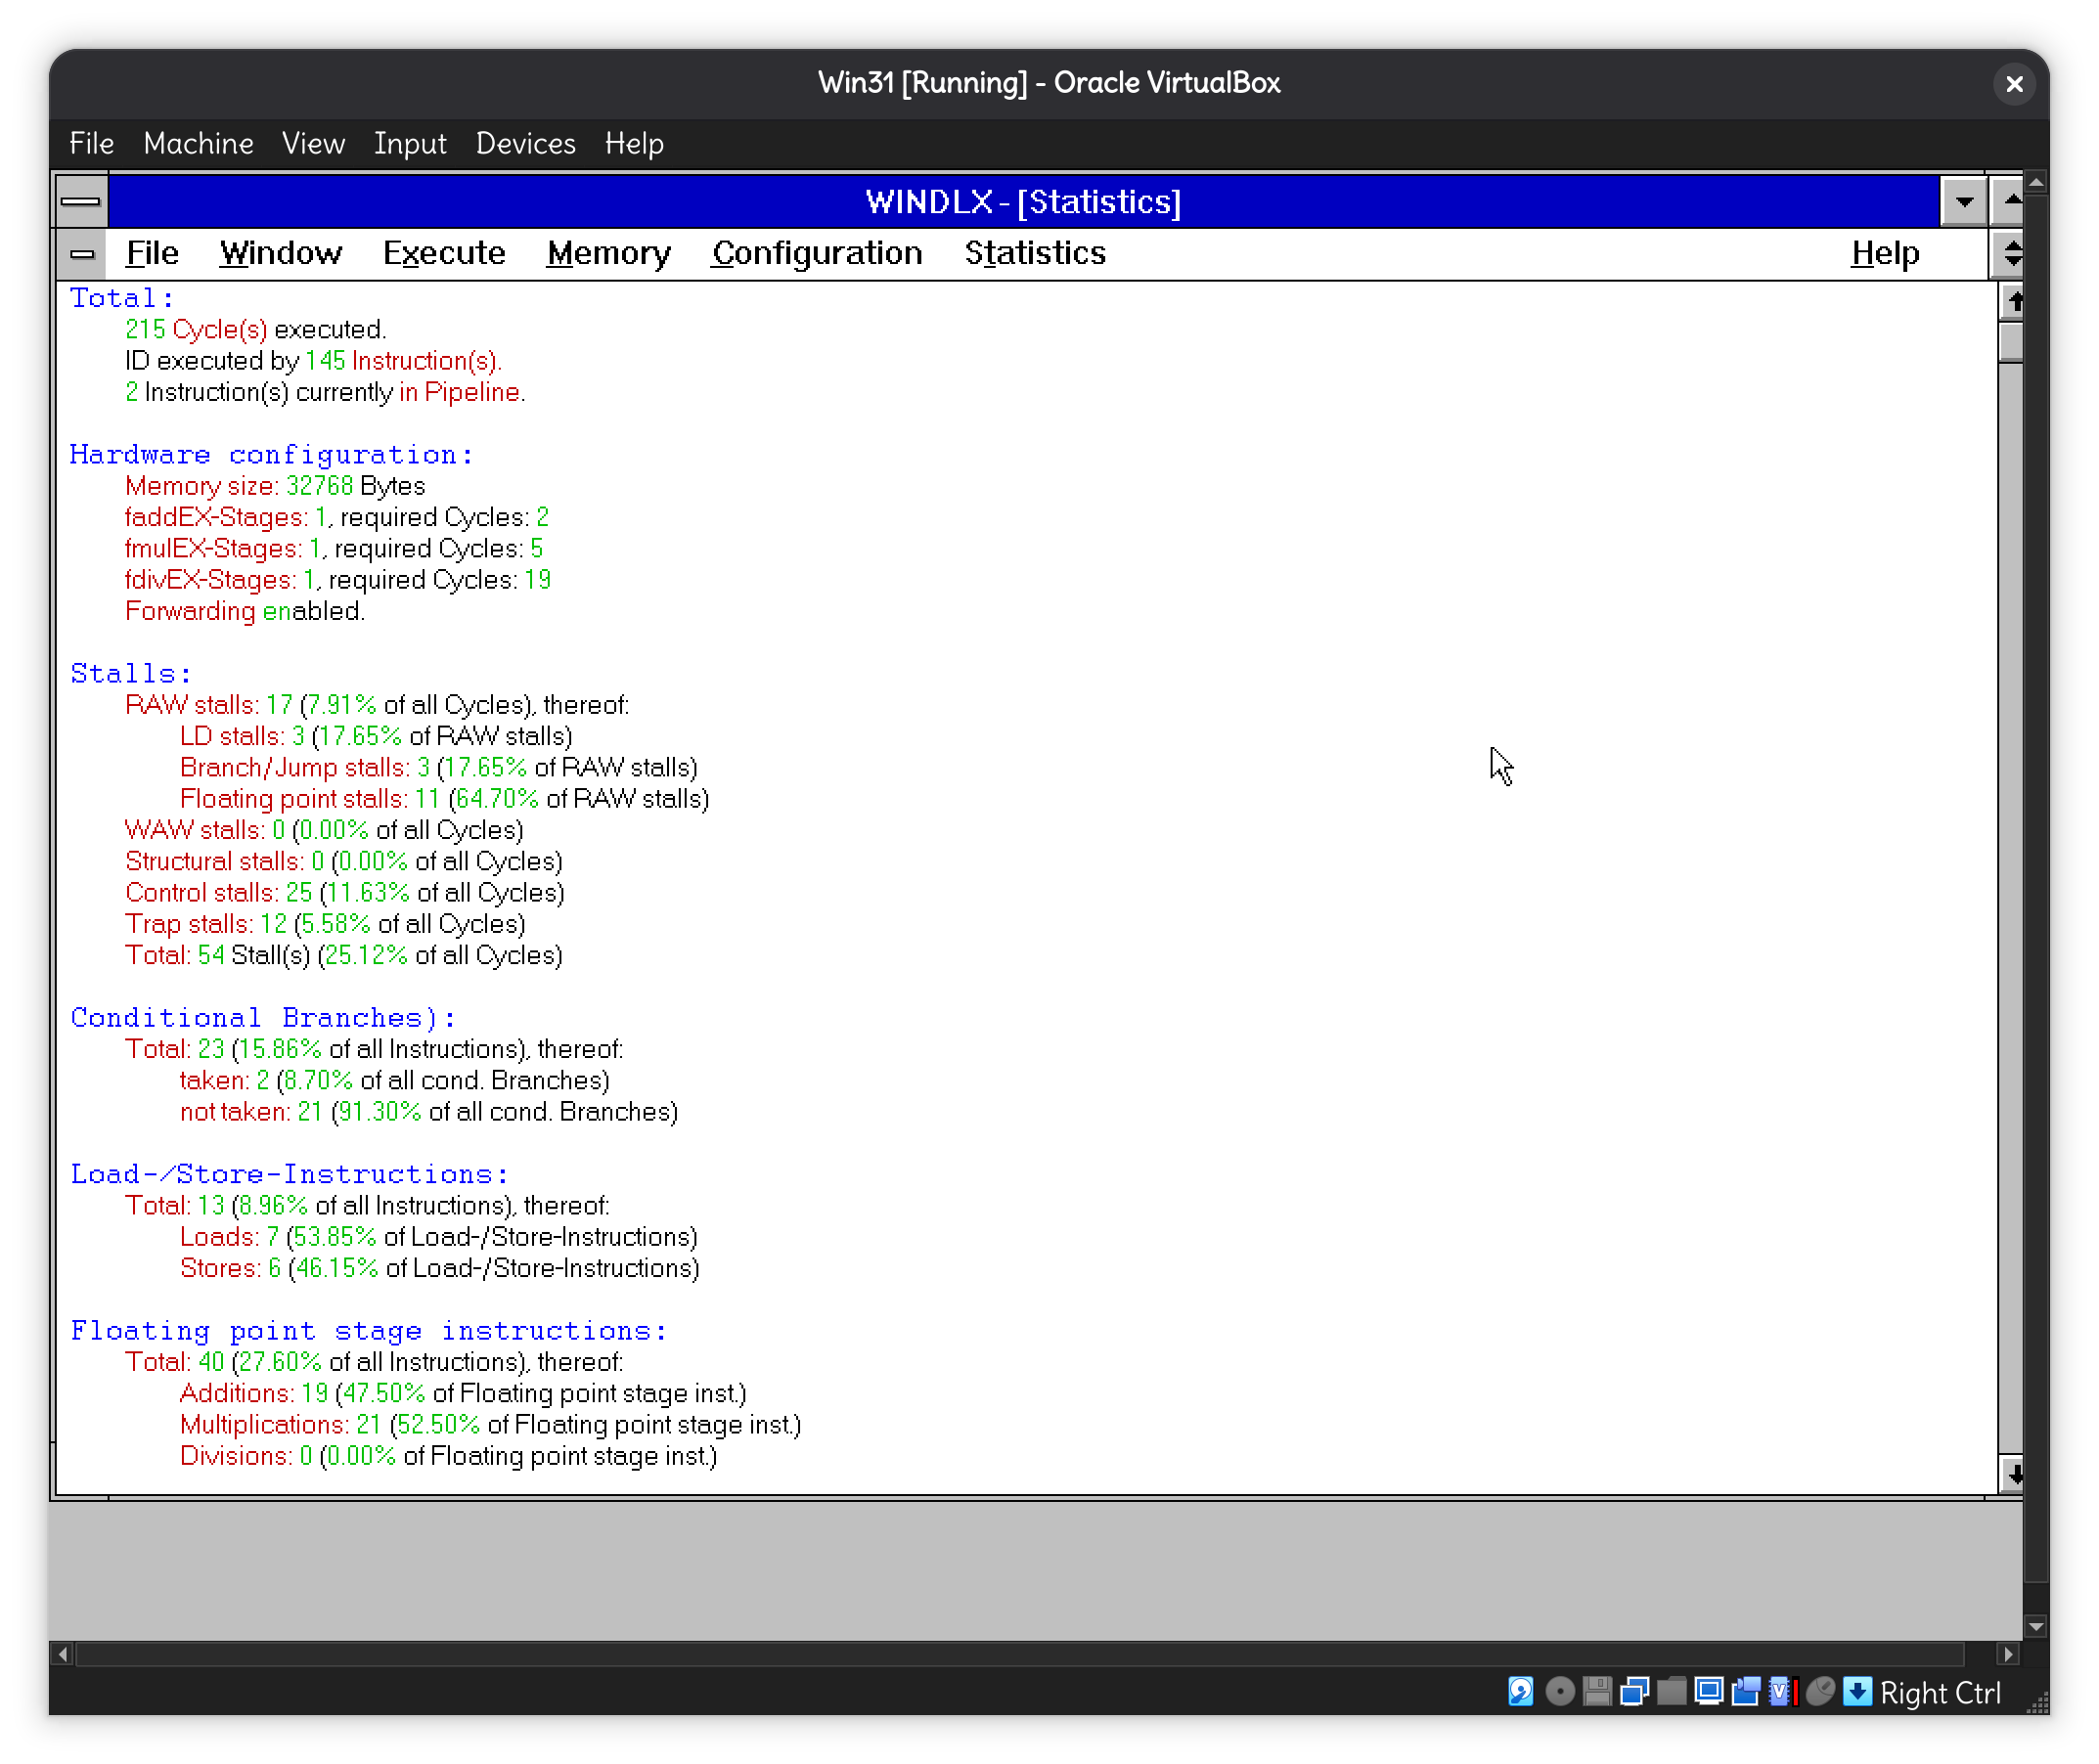
\includegraphics[width=0.9\textwidth]{images/statistics_with_forwarding.png}
\caption{WinDLX统计：Forwarding Enabled}
\label{fig:with_forwarding}
\end{figure}

\begin{figure}[H]
\centering
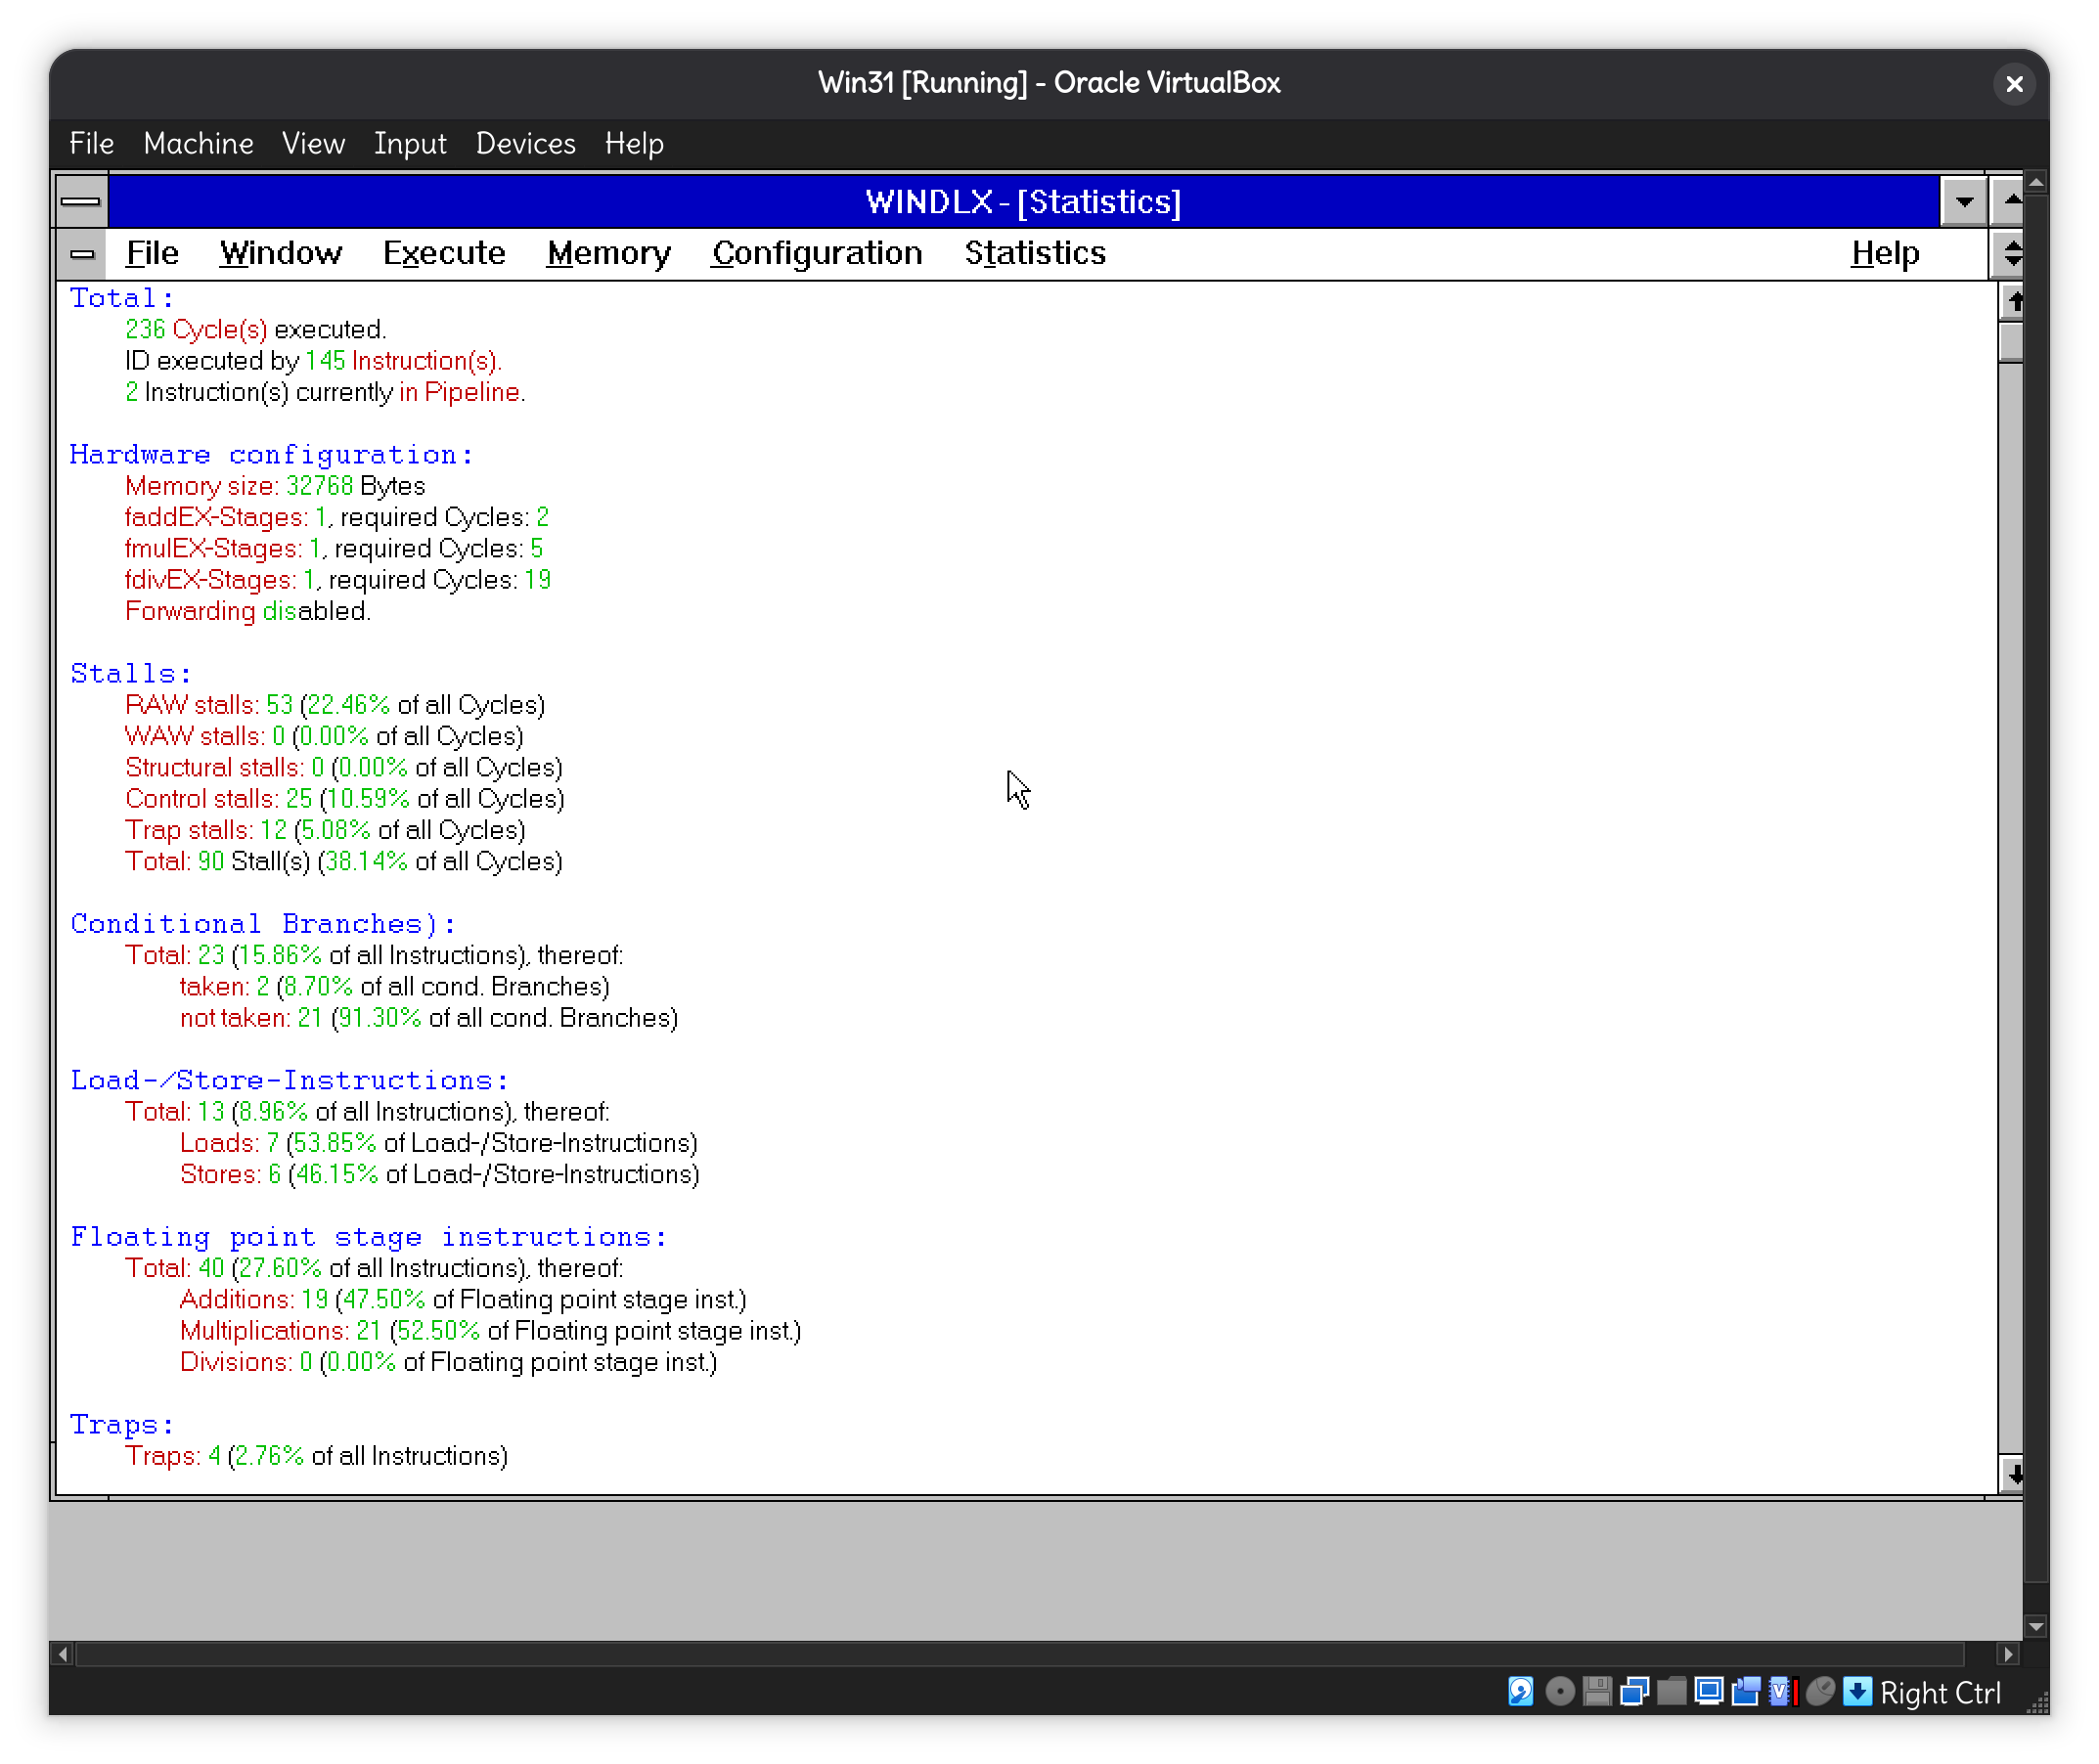
\includegraphics[width=0.9\textwidth]{images/statistics_without_forwarding.png}
\caption{WinDLX统计：Forwarding Disabled}
\label{fig:without_forwarding}
\end{figure}

对比分析：
\begin{itemize}
	\item 开启定向路径：总周期215，总停顿54（25.12\%），RAW停顿17（7.91\%）。
	\item 关闭定向路径：总周期236，总停顿90（38.14\%），RAW停顿53（22.46\%）。
	\item 在同为145条已执行指令时，开启Forwarding减少21个周期，显著降低RAW相关停顿。
\end{itemize}

\subsection{MIPSsim结果：无冲突场景}
\begin{figure}[H]
\centering
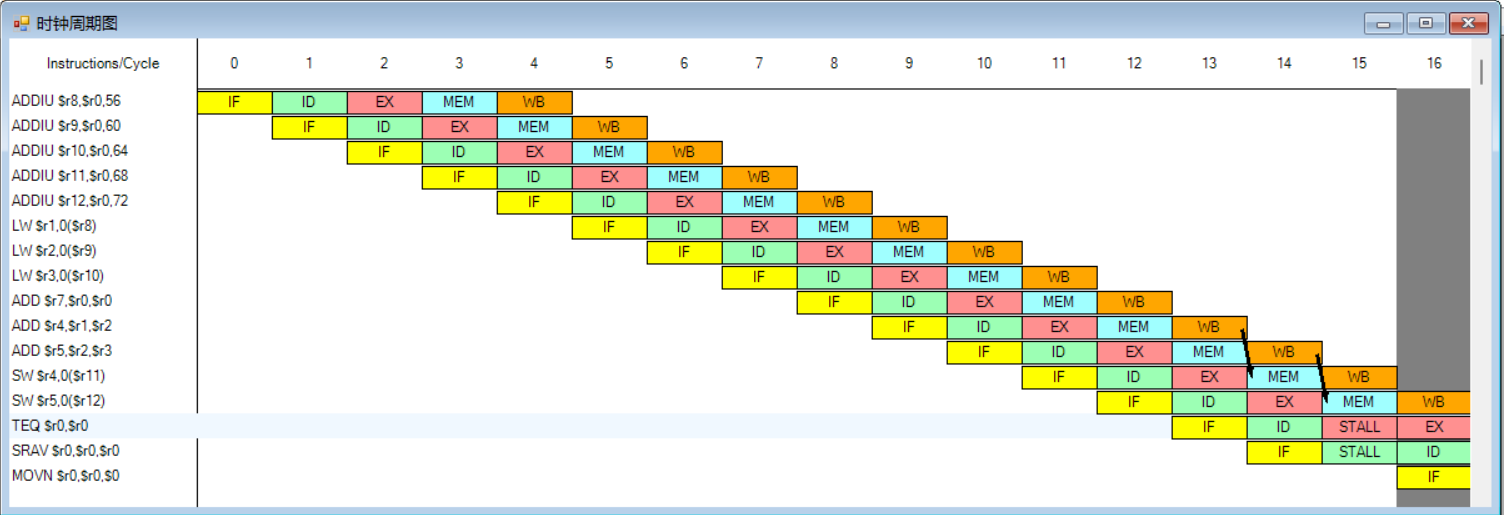
\includegraphics[width=0.95\textwidth]{images/no_hazard_cycle_diagram.png}
\caption{no\_hazard.s 时钟周期图}
\label{fig:no_hazard_cycle}
\end{figure}

\begin{figure}[H]
\centering
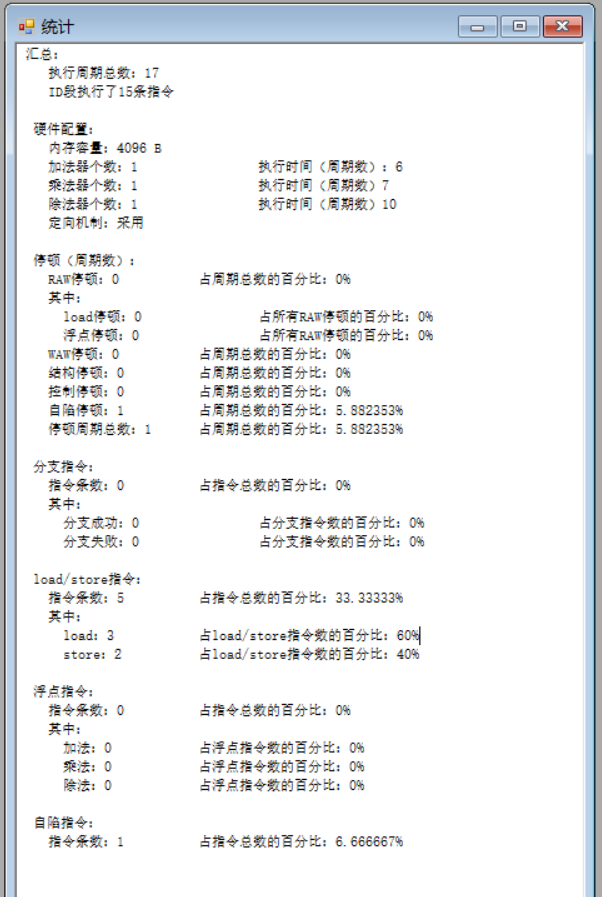
\includegraphics[width=0.58\textwidth]{images/no_hazard_statistics.png}
\caption{no\_hazard.s 统计信息}
\label{fig:no_hazard_stat}
\end{figure}

观察与分析：
\begin{itemize}
	\item 执行周期总数为17，RAW停顿为0，控制停顿为0。
	\item 仅出现程序结束相关停顿（停顿周期总数1，占5.882353\%）。
	\item 满足“无冲突流水线演示”的实验要求。
\end{itemize}

\subsection{MIPSsim结果：RAW冲突场景}
\begin{figure}[H]
\centering
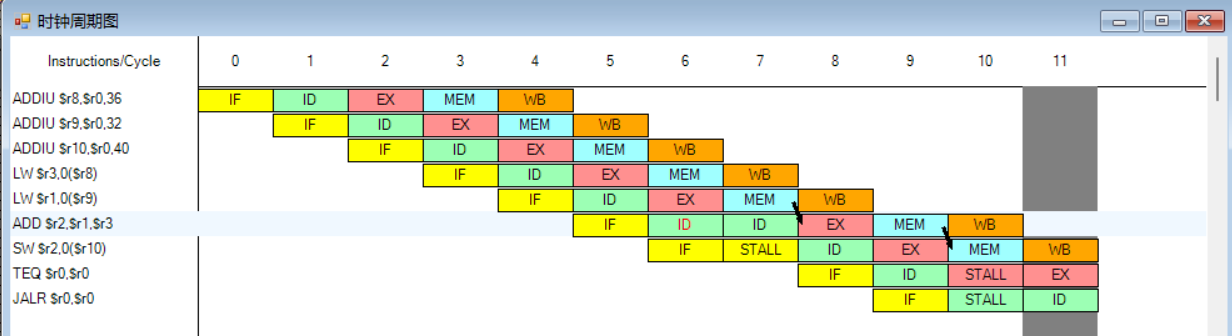
\includegraphics[width=0.95\textwidth]{images/raw_hazard_cycle_diagram.png}
\caption{raw\_hazard.s 时钟周期图}
\label{fig:raw_hazard_cycle}
\end{figure}

\begin{figure}[H]
\centering
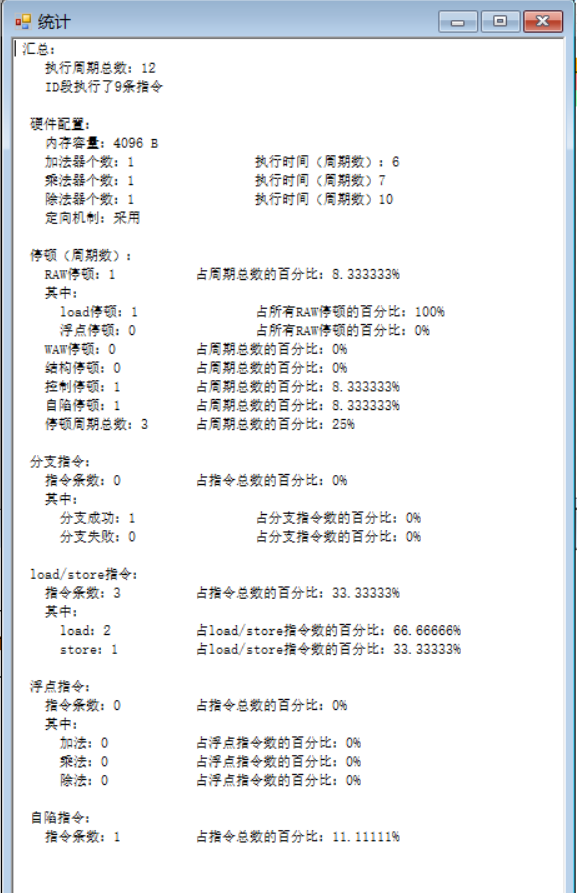
\includegraphics[width=0.58\textwidth]{images/raw_hazard_statistics.png}
\caption{raw\_hazard.s 统计信息}
\label{fig:raw_hazard_stat}
\end{figure}

观察与分析：
\begin{itemize}
	\item 执行周期总数为12，出现RAW停顿1次（均为load停顿，占所有RAW停顿100\%）。
	\item 控制停顿1次，总停顿周期3（占25\%）。
	\item 周期图中可见\texttt{ADD}前后存在明显插入停顿，符合load-use冲突机理。
\end{itemize}

\subsection{MIPSsim结果：分支跳转场景}
\begin{figure}[H]
\centering
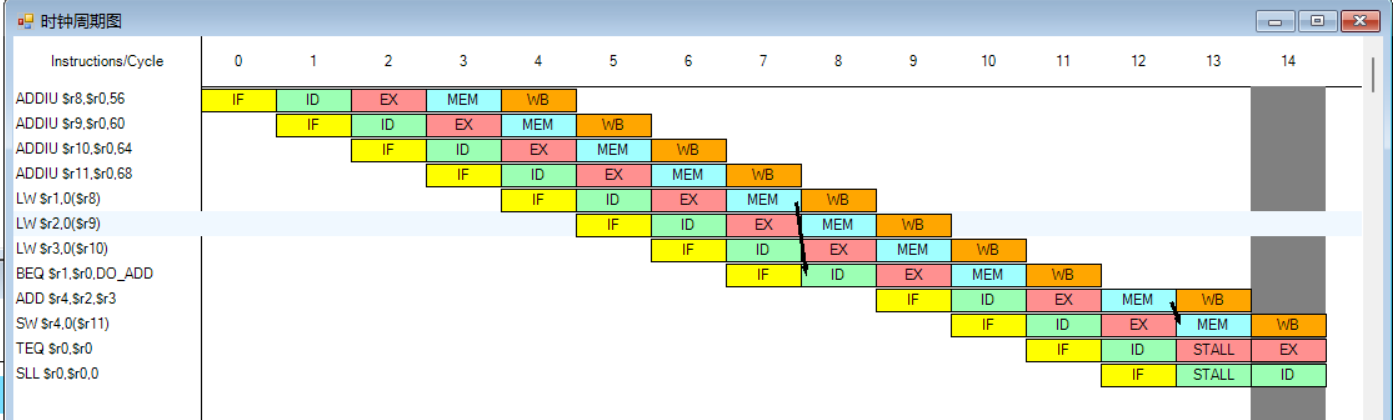
\includegraphics[width=0.95\textwidth]{images/branch_jump_cycle_diagram.png}
\caption{branch\_jump.s 时钟周期图}
\label{fig:branch_cycle}
\end{figure}

\begin{figure}[H]
\centering
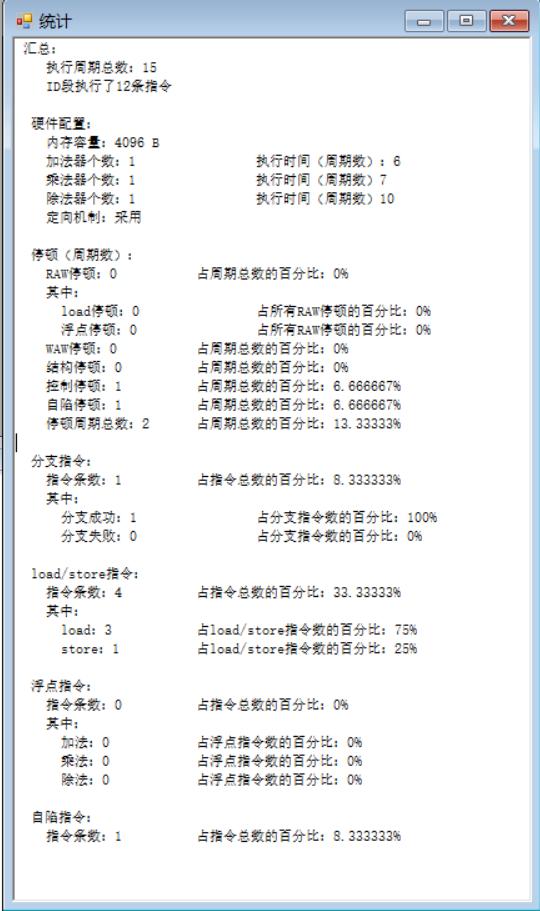
\includegraphics[width=0.58\textwidth]{images/branch_jump_statistics.png}
\caption{branch\_jump.s 统计信息}
\label{fig:branch_stat}
\end{figure}

观察与分析：
\begin{itemize}
	\item 执行周期总数为15，分支指令条数1，分支成功1次（成功率100\%）。
	\item 控制停顿1次，占总周期6.666667\%。
	\item 总停顿周期2（占13.33333\%），说明分支决策导致了流水线代价。
\end{itemize}

\section{总结}
本实验完成了实验指导书要求的性能分析和三类代码组合设计，并基于模拟器结果进行了分析：
\begin{itemize}
	\item 通过\texttt{no\_hazard.s}验证了可实现近似无数据冲突的流水执行。
	\item 通过\texttt{raw\_hazard.s}验证了load-use型RAW冲突会引入停顿。
	\item 通过\texttt{branch\_jump.s}验证了分支跳转会带来控制相关开销。
	\item 通过WinDLX对比验证了Forwarding在降低RAW停顿与总周期方面的有效性。
\end{itemize}

实验体会：在这次实验中，我掌握了MIPS模拟器的基本使用方法，更加直观地看到了程序运行过程中流水线的各个阶段。理解了流水线性能不仅取决于指令数量，还与指令编排、相关类型和硬件机制（如定向路径）紧密相关。合理调度可显著减少停顿，提高吞吐。

\section*{附录：实验源代码}
\subsection*{A.1 no\_hazard.s}
\begin{lstlisting}
.text
main:
ADDIU $r8,$r0,A
ADDIU $r9,$r0,B
ADDIU $r10,$r0,C
ADDIU $r11,$r0,RES1
ADDIU $r12,$r0,RES2
LW    $r1,0($r8)
LW    $r2,0($r9)
LW    $r3,0($r10)
ADD   $r7,$r0,$r0
ADD   $r4,$r1,$r2
ADD   $r5,$r2,$r3
SW    $r4,0($r11)
SW    $r5,0($r12)
TEQ   $r0,$r0

.data
A:    .word 7
B:    .word 11
C:    .word 5
RES1: .word 0
RES2: .word 0
\end{lstlisting}

\subsection*{A.2 raw\_hazard.s}
\begin{lstlisting}
.text
main:
ADDIU $r8,$r0,INC
ADDIU $r9,$r0,VAL
ADDIU $r10,$r0,OUT
LW    $r3,0($r8)
LW    $r1,0($r9)
ADD   $r2,$r1,$r3
SW    $r2,0($r10)
TEQ   $r0,$r0

.data
VAL:  .word 9
INC:  .word 1
OUT:  .word 0
\end{lstlisting}

\subsection*{A.3 branch\_jump.s}
\begin{lstlisting}
.text
main:
ADDIU $r8,$r0,FLAG
ADDIU $r9,$r0,X
ADDIU $r10,$r0,Y
ADDIU $r11,$r0,OUT
LW    $r1,0($r8)
LW    $r2,0($r9)
LW    $r3,0($r10)
BEQ   $r1,$r0,DO_ADD
ADD   $r4,$r0,$r0
SW    $r4,0($r11)
TEQ   $r0,$r0

DO_ADD:
ADD   $r4,$r2,$r3
SW    $r4,0($r11)
TEQ   $r0,$r0

.data
FLAG: .word 0
X:    .word 12
Y:    .word 30
OUT:  .word 0
\end{lstlisting}

\subsection*{A.4 运行说明}
\begin{verbatim}
1) 在 MIPSsim 中分别加载并运行 no_hazard.s / raw_hazard.s / branch_jump.s。
2) 打开“时钟周期图”和“统计”窗口截图。
3) 在 WinDLX 中分别开启和关闭 Forwarding，记录 Statistics 页面。
\end{verbatim}

\end{document}
